% Week 1 v2. Shared style and exact unit-edge geometry.
\usepackage[letterpaper,margin=.65in,top=.60in,bottom=.65in]{geometry}
\usepackage[T1]{fontenc}
\usepackage[default]{sourcesanspro}
\usepackage{microtype,tikz,array,tabularx,fancyhdr,amsmath}
\usepackage[hidelinks]{hyperref}
\usetikzlibrary{calc,arrows.meta}
\setlength{\parindent}{0pt}\setlength{\parskip}{7pt}
\setlength{\headheight}{0pt}\setlength{\footskip}{26pt}
\setlength{\emergencystretch}{2em}
\pagestyle{fancy}\fancyhf{}\renewcommand{\headrulewidth}{0pt}\renewcommand{\footrulewidth}{.4pt}
\fancyfoot[L]{\scriptsize Bellingham Math Circle / Week 1 / \activityid}
\fancyfoot[R]{\scriptsize \thepage}
\definecolor{ink}{gray}{.12}\definecolor{soft}{gray}{.95}\color{ink}
\newlength{\blockside}\setlength{\blockside}{1in}
\def\hh{0.8660254037844386}
\tikzset{outline/.style={draw=ink,line width=1.05pt,line join=round},tile/.style={draw=ink,line width=.65pt,line join=round},gridline/.style={draw=black!40,line width=.35pt}}
\newcommand{\HexPath}{(-1,0)--(-.5,-\hh)--(.5,-\hh)--(1,0)--(.5,\hh)--(-.5,\hh)--cycle}
\newcommand{\BluePath}{(0,0)--(1,0)--(1.5,\hh)--(.5,\hh)--cycle}
\newcommand{\ChevronPath}{(0,0)--(1,0)--(1.5,\hh)--(1,2*\hh)--(0,2*\hh)--(.5,\hh)--cycle}
\newcommand{\BoardPath}{(0,0)--(1,0)--(2,2*\hh)--(1,4*\hh)--(0,4*\hh)--(-1,2*\hh)--cycle}
\newcommand{\PageTitle}[2]{{\fontsize{10}{12}\selectfont\bfseries WEEK 1\quad TILING LAB\hfill #1\par}\vspace{3pt}{\fontsize{27}{30}\selectfont\bfseries #2\par}\vspace{2pt}}
\newcommand{\NameLine}{{\small Name: \rule{2.65in}{.4pt}\hfill Date: \rule{1.35in}{.4pt}\par}\vspace{4pt}}
\newcommand{\Task}[2]{\par\vspace{3pt}{\large\bfseries #1}\par #2\par}
\newcommand{\Subhead}[1]{\par\vspace{3pt}{\large\bfseries #1}\par}
\newcommand{\RuleBox}[1]{\par\begingroup\setlength{\fboxsep}{8pt}\colorbox{soft}{\parbox{\dimexpr\linewidth-16pt\relax}{#1}}\endgroup\par}
\newcommand{\WriteBox}[2]{\par\textbf{#1}\par\vspace{2pt}\begin{tikzpicture}\draw[black!40,line width=.5pt] (0,0) rectangle (\dimexpr\linewidth-.5pt\relax,#2);\end{tikzpicture}\par}
\newcommand{\DrawOutline}[1]{\begin{tikzpicture}[x=\blockside,y=\blockside]\draw[outline] #1;\end{tikzpicture}}
\newcommand{\Pair}[1]{\par\vspace{4pt}\begin{minipage}[t]{.485\linewidth}\centering\textbf{First filling}\par\vspace{8pt}\DrawOutline{#1}\end{minipage}\hfill\begin{minipage}[t]{.485\linewidth}\centering\textbf{Another filling}\par\vspace{8pt}\DrawOutline{#1}\end{minipage}\par}
\newcommand{\ScaleCheck}{\vfill\par\begingroup\fontsize{9}{11}\selectfont\begin{minipage}[c]{1.2in}\centering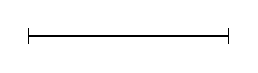
\begin{tikzpicture}[x=\blockside,y=1in]\draw[line width=.65pt] (0,0)--(1,0);\draw (0,-.04)--(0,.04) (1,-.04)--(1,.04);\end{tikzpicture}\par One small block edge\end{minipage}\hfill\begin{minipage}[c]{\dimexpr\linewidth-1.35in\relax}Adult: print \textbf{100\% / Actual Size}, single-sided. Default edge: 1 inch (25.4 mm). Compare with a \textbf{1\(\times\)} green triangle before using these mats.\end{minipage}\par\endgroup}
\newcommand{\StudentFooter}{\vfill{\small Build first. Explain by pointing, talking, or drawing.}\par}
\newcommand{\UnitRule}{Use the small (1\(\times\)) pieces. Turn them as needed.}
% An upward side-n triangle, with unit cells and no solution lines.
\newcommand{\TriangleGrid}[1]{
 \pgfmathtruncatemacro{\nn}{#1-1}
 \foreach \j in {0,...,\nn}{\pgfmathtruncatemacro{\imax}{#1-1-\j}\foreach \i in {0,...,\imax}{\draw[gridline] ({\i+.5*\j},{\hh*\j})--({\i+1+.5*\j},{\hh*\j})--({\i+.5*\j+.5},{\hh*(\j+1)})--cycle;}}
 \draw[outline] (0,0)--(#1,0)--({#1/2},{#1*\hh})--cycle;}
\newcommand{\TriangleMat}[1]{\begin{tikzpicture}[x=\blockside,y=\blockside]\TriangleGrid{#1}\end{tikzpicture}}
\newcommand{\HexBlues}{\draw[tile] \HexPath;\draw[tile] (0,0)--(1,0) (0,0)--(-.5,\hh) (0,0)--(-.5,-\hh);}
\newcommand{\FlipExample}{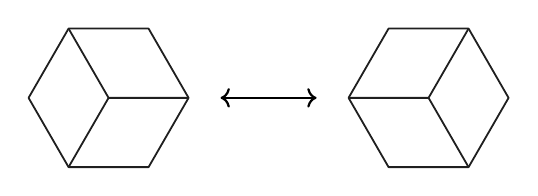
\begin{tikzpicture}[x=.40in,y=.40in]\HexBlues\begin{scope}[shift={(4,0)},rotate=60]\HexBlues\end{scope}\draw[<->,thick] (1.4,0)--(2.6,0);\end{tikzpicture}}
\newcommand{\StatePic}[2]{\begin{tikzpicture}[x=#2\blockside,y=#2\blockside]\csname Tiling#1\endcsname\draw[outline] \BoardPath;\draw[line width=2pt] (0,0)--(1,0);\end{tikzpicture}}
\newcommand{\StateCard}[1]{\begin{minipage}[t]{.30\linewidth}\centering\textbf{#1}\par\StatePic{#1}{.32}\end{minipage}}
% Generated by generate-geometry.py; coordinate unit = one small block edge.
\newcommand{\BoardGrid}{\draw[gridline] (-0.500000000,0.866025404)--(0.000000000,1.732050808)--(-1.000000000,1.732050808)--cycle;\draw[gridline] (-1.000000000,1.732050808)--(0.000000000,1.732050808)--(-0.500000000,2.598076211)--cycle;\draw[gridline] (0.000000000,1.732050808)--(0.500000000,2.598076211)--(-0.500000000,2.598076211)--cycle;\draw[gridline] (-0.500000000,2.598076211)--(0.500000000,2.598076211)--(0.000000000,3.464101615)--cycle;\draw[gridline] (0.500000000,2.598076211)--(1.000000000,3.464101615)--(0.000000000,3.464101615)--cycle;\draw[gridline] (0.000000000,0.000000000)--(0.500000000,0.866025404)--(-0.500000000,0.866025404)--cycle;\draw[gridline] (-0.500000000,0.866025404)--(0.500000000,0.866025404)--(0.000000000,1.732050808)--cycle;\draw[gridline] (0.500000000,0.866025404)--(1.000000000,1.732050808)--(0.000000000,1.732050808)--cycle;\draw[gridline] (0.000000000,1.732050808)--(1.000000000,1.732050808)--(0.500000000,2.598076211)--cycle;\draw[gridline] (1.000000000,1.732050808)--(1.500000000,2.598076211)--(0.500000000,2.598076211)--cycle;\draw[gridline] (0.500000000,2.598076211)--(1.500000000,2.598076211)--(1.000000000,3.464101615)--cycle;\draw[gridline] (0.000000000,0.000000000)--(1.000000000,0.000000000)--(0.500000000,0.866025404)--cycle;\draw[gridline] (1.000000000,0.000000000)--(1.500000000,0.866025404)--(0.500000000,0.866025404)--cycle;\draw[gridline] (0.500000000,0.866025404)--(1.500000000,0.866025404)--(1.000000000,1.732050808)--cycle;\draw[gridline] (1.500000000,0.866025404)--(2.000000000,1.732050808)--(1.000000000,1.732050808)--cycle;\draw[gridline] (1.000000000,1.732050808)--(2.000000000,1.732050808)--(1.500000000,2.598076211)--cycle;}
\newcommand{\TilingA}{\draw[tile] (-0.500000000,0.866025404)--(0.000000000,1.732050808)--(-0.500000000,2.598076211)--(-1.000000000,1.732050808)--cycle;\draw[tile] (0.000000000,1.732050808)--(0.500000000,2.598076211)--(0.000000000,3.464101615)--(-0.500000000,2.598076211)--cycle;\draw[tile] (0.500000000,2.598076211)--(1.500000000,2.598076211)--(1.000000000,3.464101615)--(0.000000000,3.464101615)--cycle;\draw[tile] (0.000000000,0.000000000)--(0.500000000,0.866025404)--(0.000000000,1.732050808)--(-0.500000000,0.866025404)--cycle;\draw[tile] (0.500000000,0.866025404)--(1.000000000,1.732050808)--(0.500000000,2.598076211)--(0.000000000,1.732050808)--cycle;\draw[tile] (1.000000000,1.732050808)--(2.000000000,1.732050808)--(1.500000000,2.598076211)--(0.500000000,2.598076211)--cycle;\draw[tile] (0.000000000,0.000000000)--(1.000000000,0.000000000)--(1.500000000,0.866025404)--(0.500000000,0.866025404)--cycle;\draw[tile] (0.500000000,0.866025404)--(1.500000000,0.866025404)--(2.000000000,1.732050808)--(1.000000000,1.732050808)--cycle;}
\newcommand{\PathA}{\draw[-{Stealth[length=4pt]},line width=1.2pt,dashed] (0.500000000,0.000000000)--(1.000000000,0.866025404);\draw[-{Stealth[length=4pt]},line width=1.2pt,dashed] (1.000000000,0.866025404)--(1.500000000,1.732050808);\draw[-{Stealth[length=4pt]},line width=1.2pt,dashed] (1.500000000,1.732050808)--(1.000000000,2.598076211);\draw[-{Stealth[length=4pt]},line width=1.2pt,dashed] (1.000000000,2.598076211)--(0.500000000,3.464101615);}
\newcommand{\TilingB}{\draw[tile] (-0.500000000,0.866025404)--(0.000000000,1.732050808)--(-0.500000000,2.598076211)--(-1.000000000,1.732050808)--cycle;\draw[tile] (0.000000000,1.732050808)--(0.500000000,2.598076211)--(0.000000000,3.464101615)--(-0.500000000,2.598076211)--cycle;\draw[tile] (0.500000000,2.598076211)--(1.500000000,2.598076211)--(1.000000000,3.464101615)--(0.000000000,3.464101615)--cycle;\draw[tile] (0.000000000,0.000000000)--(0.500000000,0.866025404)--(0.000000000,1.732050808)--(-0.500000000,0.866025404)--cycle;\draw[tile] (0.500000000,0.866025404)--(1.500000000,0.866025404)--(1.000000000,1.732050808)--(0.000000000,1.732050808)--cycle;\draw[tile] (0.000000000,1.732050808)--(1.000000000,1.732050808)--(1.500000000,2.598076211)--(0.500000000,2.598076211)--cycle;\draw[tile] (0.000000000,0.000000000)--(1.000000000,0.000000000)--(1.500000000,0.866025404)--(0.500000000,0.866025404)--cycle;\draw[tile] (1.500000000,0.866025404)--(2.000000000,1.732050808)--(1.500000000,2.598076211)--(1.000000000,1.732050808)--cycle;}
\newcommand{\PathB}{\draw[-{Stealth[length=4pt]},line width=1.2pt,dashed] (0.500000000,0.000000000)--(1.000000000,0.866025404);\draw[-{Stealth[length=4pt]},line width=1.2pt,dashed] (1.000000000,0.866025404)--(0.500000000,1.732050808);\draw[-{Stealth[length=4pt]},line width=1.2pt,dashed] (0.500000000,1.732050808)--(1.000000000,2.598076211);\draw[-{Stealth[length=4pt]},line width=1.2pt,dashed] (1.000000000,2.598076211)--(0.500000000,3.464101615);}
\newcommand{\TilingC}{\draw[tile] (-0.500000000,0.866025404)--(0.000000000,1.732050808)--(-0.500000000,2.598076211)--(-1.000000000,1.732050808)--cycle;\draw[tile] (0.000000000,1.732050808)--(0.500000000,2.598076211)--(0.000000000,3.464101615)--(-0.500000000,2.598076211)--cycle;\draw[tile] (0.500000000,2.598076211)--(1.500000000,2.598076211)--(1.000000000,3.464101615)--(0.000000000,3.464101615)--cycle;\draw[tile] (0.000000000,0.000000000)--(1.000000000,0.000000000)--(0.500000000,0.866025404)--(-0.500000000,0.866025404)--cycle;\draw[tile] (-0.500000000,0.866025404)--(0.500000000,0.866025404)--(1.000000000,1.732050808)--(0.000000000,1.732050808)--cycle;\draw[tile] (0.000000000,1.732050808)--(1.000000000,1.732050808)--(1.500000000,2.598076211)--(0.500000000,2.598076211)--cycle;\draw[tile] (1.000000000,0.000000000)--(1.500000000,0.866025404)--(1.000000000,1.732050808)--(0.500000000,0.866025404)--cycle;\draw[tile] (1.500000000,0.866025404)--(2.000000000,1.732050808)--(1.500000000,2.598076211)--(1.000000000,1.732050808)--cycle;}
\newcommand{\PathC}{\draw[-{Stealth[length=4pt]},line width=1.2pt,dashed] (0.500000000,0.000000000)--(0.000000000,0.866025404);\draw[-{Stealth[length=4pt]},line width=1.2pt,dashed] (0.000000000,0.866025404)--(0.500000000,1.732050808);\draw[-{Stealth[length=4pt]},line width=1.2pt,dashed] (0.500000000,1.732050808)--(1.000000000,2.598076211);\draw[-{Stealth[length=4pt]},line width=1.2pt,dashed] (1.000000000,2.598076211)--(0.500000000,3.464101615);}
\newcommand{\TilingD}{\draw[tile] (-0.500000000,0.866025404)--(0.000000000,1.732050808)--(-0.500000000,2.598076211)--(-1.000000000,1.732050808)--cycle;\draw[tile] (0.000000000,1.732050808)--(1.000000000,1.732050808)--(0.500000000,2.598076211)--(-0.500000000,2.598076211)--cycle;\draw[tile] (-0.500000000,2.598076211)--(0.500000000,2.598076211)--(1.000000000,3.464101615)--(0.000000000,3.464101615)--cycle;\draw[tile] (0.000000000,0.000000000)--(0.500000000,0.866025404)--(0.000000000,1.732050808)--(-0.500000000,0.866025404)--cycle;\draw[tile] (0.500000000,0.866025404)--(1.500000000,0.866025404)--(1.000000000,1.732050808)--(0.000000000,1.732050808)--cycle;\draw[tile] (1.000000000,1.732050808)--(1.500000000,2.598076211)--(1.000000000,3.464101615)--(0.500000000,2.598076211)--cycle;\draw[tile] (0.000000000,0.000000000)--(1.000000000,0.000000000)--(1.500000000,0.866025404)--(0.500000000,0.866025404)--cycle;\draw[tile] (1.500000000,0.866025404)--(2.000000000,1.732050808)--(1.500000000,2.598076211)--(1.000000000,1.732050808)--cycle;}
\newcommand{\PathD}{\draw[-{Stealth[length=4pt]},line width=1.2pt,dashed] (0.500000000,0.000000000)--(1.000000000,0.866025404);\draw[-{Stealth[length=4pt]},line width=1.2pt,dashed] (1.000000000,0.866025404)--(0.500000000,1.732050808);\draw[-{Stealth[length=4pt]},line width=1.2pt,dashed] (0.500000000,1.732050808)--(0.000000000,2.598076211);\draw[-{Stealth[length=4pt]},line width=1.2pt,dashed] (0.000000000,2.598076211)--(0.500000000,3.464101615);}
\newcommand{\TilingE}{\draw[tile] (-0.500000000,0.866025404)--(0.000000000,1.732050808)--(-0.500000000,2.598076211)--(-1.000000000,1.732050808)--cycle;\draw[tile] (0.000000000,1.732050808)--(1.000000000,1.732050808)--(0.500000000,2.598076211)--(-0.500000000,2.598076211)--cycle;\draw[tile] (-0.500000000,2.598076211)--(0.500000000,2.598076211)--(1.000000000,3.464101615)--(0.000000000,3.464101615)--cycle;\draw[tile] (0.000000000,0.000000000)--(1.000000000,0.000000000)--(0.500000000,0.866025404)--(-0.500000000,0.866025404)--cycle;\draw[tile] (-0.500000000,0.866025404)--(0.500000000,0.866025404)--(1.000000000,1.732050808)--(0.000000000,1.732050808)--cycle;\draw[tile] (1.000000000,1.732050808)--(1.500000000,2.598076211)--(1.000000000,3.464101615)--(0.500000000,2.598076211)--cycle;\draw[tile] (1.000000000,0.000000000)--(1.500000000,0.866025404)--(1.000000000,1.732050808)--(0.500000000,0.866025404)--cycle;\draw[tile] (1.500000000,0.866025404)--(2.000000000,1.732050808)--(1.500000000,2.598076211)--(1.000000000,1.732050808)--cycle;}
\newcommand{\PathE}{\draw[-{Stealth[length=4pt]},line width=1.2pt,dashed] (0.500000000,0.000000000)--(0.000000000,0.866025404);\draw[-{Stealth[length=4pt]},line width=1.2pt,dashed] (0.000000000,0.866025404)--(0.500000000,1.732050808);\draw[-{Stealth[length=4pt]},line width=1.2pt,dashed] (0.500000000,1.732050808)--(0.000000000,2.598076211);\draw[-{Stealth[length=4pt]},line width=1.2pt,dashed] (0.000000000,2.598076211)--(0.500000000,3.464101615);}
\newcommand{\TilingF}{\draw[tile] (-0.500000000,0.866025404)--(0.500000000,0.866025404)--(0.000000000,1.732050808)--(-1.000000000,1.732050808)--cycle;\draw[tile] (-1.000000000,1.732050808)--(0.000000000,1.732050808)--(0.500000000,2.598076211)--(-0.500000000,2.598076211)--cycle;\draw[tile] (-0.500000000,2.598076211)--(0.500000000,2.598076211)--(1.000000000,3.464101615)--(0.000000000,3.464101615)--cycle;\draw[tile] (0.000000000,0.000000000)--(1.000000000,0.000000000)--(0.500000000,0.866025404)--(-0.500000000,0.866025404)--cycle;\draw[tile] (0.500000000,0.866025404)--(1.000000000,1.732050808)--(0.500000000,2.598076211)--(0.000000000,1.732050808)--cycle;\draw[tile] (1.000000000,1.732050808)--(1.500000000,2.598076211)--(1.000000000,3.464101615)--(0.500000000,2.598076211)--cycle;\draw[tile] (1.000000000,0.000000000)--(1.500000000,0.866025404)--(1.000000000,1.732050808)--(0.500000000,0.866025404)--cycle;\draw[tile] (1.500000000,0.866025404)--(2.000000000,1.732050808)--(1.500000000,2.598076211)--(1.000000000,1.732050808)--cycle;}
\newcommand{\PathF}{\draw[-{Stealth[length=4pt]},line width=1.2pt,dashed] (0.500000000,0.000000000)--(0.000000000,0.866025404);\draw[-{Stealth[length=4pt]},line width=1.2pt,dashed] (0.000000000,0.866025404)--(-0.500000000,1.732050808);\draw[-{Stealth[length=4pt]},line width=1.2pt,dashed] (-0.500000000,1.732050808)--(0.000000000,2.598076211);\draw[-{Stealth[length=4pt]},line width=1.2pt,dashed] (0.000000000,2.598076211)--(0.500000000,3.464101615);}
\newcommand{\TriangleSolution}{\draw[tile,fill=white] (0.000000000,0.000000000)--(1.000000000,0.000000000)--(1.500000000,0.866025404)--(0.500000000,0.866025404)--cycle;\node[font=\small] at (0.750000000,0.433012702) {B};\draw[tile,fill=white] (1.000000000,0.000000000)--(2.000000000,0.000000000)--(2.500000000,0.866025404)--(1.500000000,0.866025404)--cycle;\node[font=\small] at (1.750000000,0.433012702) {B};\draw[tile,fill=white] (0.500000000,0.866025404)--(1.500000000,0.866025404)--(2.000000000,1.732050808)--(1.000000000,1.732050808)--cycle;\node[font=\small] at (1.250000000,1.299038106) {B};\draw[tile,fill=black!12] (2.000000000,0.000000000)--(3.000000000,0.000000000)--(2.500000000,0.866025404)--cycle;\node[font=\small] at (2.500000000,0.288675135) {G};\draw[tile,fill=black!12] (1.500000000,0.866025404)--(2.500000000,0.866025404)--(2.000000000,1.732050808)--cycle;\node[font=\small] at (2.000000000,1.154700538) {G};\draw[tile,fill=black!12] (1.000000000,1.732050808)--(2.000000000,1.732050808)--(1.500000000,2.598076211)--cycle;\node[font=\small] at (1.500000000,2.020725942) {G};}
\newcommand{\TrianglePurpleSolution}{\draw[tile,fill=white] (1.000000000,0.000000000)--(2.000000000,0.000000000)--(2.500000000,0.866025404)--(2.000000000,1.732050808)--(1.000000000,1.732050808)--(1.500000000,0.866025404)--cycle;\node[font=\small] at (1.950000000,0.866025404) {P};\draw[tile,fill=white] (0.000000000,0.000000000)--(1.000000000,0.000000000)--(1.500000000,0.866025404)--(0.500000000,0.866025404)--cycle;\node[font=\small] at (0.750000000,0.433012702) {B};\draw[tile,fill=black!12] (0.500000000,0.866025404)--(1.500000000,0.866025404)--(1.000000000,1.732050808)--cycle;\node[font=\small] at (1.000000000,1.154700538) {G};\draw[tile,fill=black!12] (1.000000000,1.732050808)--(2.000000000,1.732050808)--(1.500000000,2.598076211)--cycle;\node[font=\small] at (1.500000000,2.020725942) {G};\draw[tile,fill=black!12] (2.000000000,0.000000000)--(3.000000000,0.000000000)--(2.500000000,0.866025404)--cycle;\node[font=\small] at (2.500000000,0.288675135) {G};}
\newcommand{\Bottleneck}{\draw[tile] (0.000000000,0.000000000)--(1.000000000,0.000000000)--(0.500000000,0.866025404)--cycle;\node[font=\bfseries\small] at (0.500000000,0.288675135) {A};\draw[tile] (1.000000000,0.000000000)--(2.000000000,0.000000000)--(1.500000000,0.866025404)--cycle;\node[font=\bfseries\small] at (1.500000000,0.288675135) {B};\draw[tile] (0.500000000,0.866025404)--(1.500000000,0.866025404)--(1.000000000,1.732050808)--cycle;\node[font=\bfseries\small] at (1.000000000,1.154700538) {C};\draw[tile] (1.500000000,0.866025404)--(1.000000000,0.000000000)--(0.500000000,0.866025404)--cycle;\node[font=\bfseries\small] at (1.000000000,0.577350269) {D};\draw[tile] (1.000000000,1.732050808)--(0.500000000,0.866025404)--(0.000000000,1.732050808)--cycle;\node[font=\bfseries\small] at (0.500000000,1.443375673) {E};\draw[tile] (2.000000000,1.732050808)--(1.500000000,0.866025404)--(1.000000000,1.732050808)--cycle;\node[font=\bfseries\small] at (1.500000000,1.443375673) {F};}

